\chapter[Математическая теория кодов аутентификации]{Математическая
теория кодов аутентификации}
Сюда мы включаем и цифровые подписи и коды–имитовставки.
Стойкость кодов аутентификации базируется на:

\begin{itemize}
\item вычислительной стойкости (это очень очень сложно)
\item доказуемая стойкость (сведение к признанно сложной задаче)
\item безусловная стойкость (недостаточно информации для взлома)
\end{itemize}
Участники процесса аутентификации:

\begin{itemize}
\item отправитель $A$ (Алиса)
\item получатель $B$ (Боб) ($A$ и $B$ могут быть одним лицом)
\item криптоаналитик $Kr$ (Крамер) 
\item арбитр $Ar$ (Арнольд) (требуется в некоторых случаях)
\end{itemize}
\section{Построение кода аутентификации ($A$-кода)
(математическая модель)}

Пусть $S$ --- источник информации, который наблюдается $A$.

$S=\left\{{s}_{i} \mid i=1{\dots}\left|S\right|\right\}$  --–  эти сообщения
надо передать с аутентификацией

$M=\left\{{m}_{i} \mid i=1{\dots}\left|\text{М}\right|\right\}$ –-- множество
сообщений, полученных в результате кодирования

$E=\left\{{e}_{i} \mid i=1{\dots}\left|E\right|\right\}$ --– множество
алгоритмов кодирования с аутентификацией: 
${\forall}i:{e}_{i}:S\rightarrow M$

На все  ${e}_{i}$ распространяются такие условия:
\begin{enumerate}
\item\label{it:properties:e:inj}
  ${e}_{i}$ --- инъекция, однако может быть многозначной (в этом
  случае инъективность понимается в том смысле, что образы различных
  входов не пересекаются).
  Будем считать, что  $M=\bigcup\limits_{e \in E} e\left( S \right)$
  --– объединение $e\left( S \right)$
\item\label{it:properties:e:inv}
  Существет обратное отображение.
  Для  ${\forall}e \in S$ определим обратное отображение
  \begin{equation*}
    {f}_{e}:M\rightarrow S \cup \left\{ 0 \right\}
  \end{equation*}
  То есть
  \begin{equation*}
    \begin{cases}
      \forall s \in S, e \in E&: {f}_{e}\left(e\left(s\right)\right)=S,\\
      \forall m \notin e\left( S \right)&: {f}_{e}\left(m\right)=0.
    \end{cases}
  \end{equation*}
\end{enumerate}


\begin{example}
  Если $e$ –-- алгоритм шифрования с ключом $K$, то  ${f}_{e} = ?$
  --- алгоритм шифрования на том же ключе.
\end{example}

Код аутентификации --– тройка $AK = <S, E, M>$, где 
\begin{itemize}
  \item
    $S$ --- множество сообщений (открытых текстов) = состояний источника
сообщений
  \item
    $E$ --– множество кодов $e:S\rightarrow M$
  \item
    $M$ --– множество сообщений для передачи (закодированных сообщений) и
    выполняются условия \ref{it:properties:e:inj} и \ref{it:properties:e:inv}
    для отображений $e$
\end{itemize}

 Свойства:

\begin{itemize}
  \item
    Множество кодов $E$ --- открытая информация и известна аналитику
  \item
    $A$ и $B$ предварительно строят $A$-код и выбирают из множества $E$
    случайное отображение для работы --- и выбранное отображение является
    секретом (общим секретом $A$ и $B$)
  \item
    Для передачи информации о состоянии источника $S$ $A$ вычисляет 
    $m = e\left( s \right)$ --– сообщение с аутентификацией; $m$ передается $B$
  \item
    Критерий аутентичности сообщения, который применяет $B$:

    ${f}_{e}\left(m\right){\neq}0$ --- сообщение подлинно

    ${f}_{e}\left(m\right)=0$ --- сообщение не подтверждено
\end{itemize}

Дополнительные свойства

\begin{itemize}
  \item
    $\left|M\right|{\geq}\left|S\right|$ (из инъективности)
  \item 
    если $\left|M\right|=\left|S\right|$, то 
    \begin{equation*}
       \left(\forall m \in M\right) \left(\forall e \in E\right)
       \left(\nexists s \in S\right): e\left(s\right)=m
    \end{equation*}
    по сути это приведёт к тому, что все сообщения будут аутентичними и
    сама схема не пройдет
  \item
    $\left|M\right|>\left|S\right|$ (обычно даже
    $\left|M\right|{\gg}\left|S\right|$)
  \item
    Пусть
    \begin{equation*}
      E\left( m \right)
      = \left\{e \mid m \in e\left(S\right)\right\}
      =\left\{e \mid \exists s:e\left(s\right)
      =m\right\}
    \end{equation*}

    Если  $\left|E(m)\right|=1$, то всё, аналитик сразу нашел правильное $e$
    $\Rightarrow $ всё взломано.
    Отсюда новое условие на $A$-код: 
    ${\forall}m:\left|E\left(m\right)\right|>1$.

    С другой стороны, если  $\left|E\left(m\right)\right|=\left|E\right|$,
    то любое сообщение подойдет как правильное, так как
    \begin{equation*}
      \left(\forall e\right)\left(\exists s\right):e\left(s\right)=m.
    \end{equation*}
    Криптоаналитик тогда может найти ложное сообщение из множества
    $\bigcap\limits_{e{\in}E}e\left( S \right)$ 
    Уточнение к написанному (и новое условие на $A$-код) 
    \begin{equation*}
      {\forall}m:\left|E\left( m \right)\right|<\left|E\right|
    \end{equation*}
  \item
    Если $\bigcap\limits_{e{\in}E\left( m \right)} e\left( S \right) > 1$,
    то аналитик всегда сможет подобрать ложные сообщения, которые будут
    трактоваться как правильные (подделка).
    Отсюда следует последнее, пятое условие на А-код:
    \begin{equation*}
      \bigcap\limits_{e{\in}E\left( m \right)}e\left( S \right)
      = \left\{ m \right\}
    \end{equation*}
\end{itemize}

\begin{example}
Если $e$ --- многозначная функция, то $A$-код называется кодом с расщеплением
(если однозначная, то код без расщепления).

Задать $A$-код можно матрицей  $\left|E\right|\times \left|M\right|$ ---
матрицей $A$-кода.

Пусть $S = \left\{ H, T \right\}$,
$M=\left\{{m}_{1},{m}_{2},{m}_{3},{m}_{4}\right\}$,
$E=\left\{{e}_{1},{e}_{2},{e}_{3},{e}_{4}\right\}$.

Расщепление: ${e}_{3}\left(H\right)=\left\{{m}_{2}, {m}_{3}\right\}$

\begin{center}
  \begin{tabular}{|*{5}{c|}}
    \hline
    \backslashbox{e}{m} & $m_1$ & $m_2$ & $m_3$ & $m_4$ \\
    \hline
    $e_1$               &  $H$  &  $T$  &  $0$  &  $0$  \\
    \hline              
    $e_2$               &  $H$  &  $0$  &  $T$  &  $0$  \\
    \hline              
    $e_3$               &  $0$  &  $H$  &  $H$  &  $T$  \\
    \hline              
    $e_4$               &  $0$  &  $0$  &  $T$  &  $H$  \\
    \hline
  \end{tabular}
\end{center}

Если в каком-то столбике будет только один символ (как в  ${m}_{1}$, то
это будет код без секрета --- аналитик узнает, какое было сообщение,
однако оно всё равно будет аутентифицировано. 

Проверим выполнение всех условий:

\begin{enumerate}
  \item
    Условие
    \begin{equation*}
      M=\bigcup\limits_{e}\left(S\right)
    \end{equation*}
    Проверим
    \begin{equation*}
      \begin{split}
        {e}_{1}\left(S\right)&=\left\{{m}_{1},{m}_{2}\right\} \\
        {e}_{2}\left(S\right)&=\left\{{m}_{1},{m}_{3}\right\} \\
        {e}_{3}\left(S\right)&=\left\{{m}_{2},{m}_{3},{m}_{4}\right\} \\
        {e}_{4}\left(S\right)&=\left\{{m}_{3},{m}_{4}\right\}
      \end{split}
    \end{equation*}
    выполняется.
  \item
    ${\forall}s:{f}_{e}\left(e\left(s\right)\right)=s$ --- выполняется
  по построению.
  \item
    $\left|M\right| > \left| S \right|$ --- выполняется.
  \item
    Условие
    \begin{equation*}
      {\forall}m:\left|E\right|>\left|E\left(m\right)\right|>1
    \end{equation*}
    Проверка
    \begin{equation*}
      \begin{split}
        E\left({m}_{1}\right)&=\left\{{e}_{1},{e}_{2}\right\} \\
        E\left({m}_{2}\right)&=\left\{{e}_{1},{e}_{3}\right\} \\
        E\left({m}_{3}\right)&=\left\{{e}_{2},{e}_{3},{e}_{4}\right\} \\
        E\left({m}_{4}\right)&=\left\{{e}_{3},{e}_{4}\right\} \\
      \end{split}
    \end{equation*}
    выполняется.
  \item
    Условие
    \begin{equation*}
      {\forall}m: \bigcap\limits_{e \in E\left( m \right)} e\left( S \right)
                  = \left\{m\right\}
    \end{equation*}
    Проверка
  \begin{equation*}
    \begin{split}
      &{m}_{1}:{e}_{1}\left(S\right) \cap {e}_{2}\left(S\right)
      =\left\{{m}_{1}\right\} \\
      &{m}_{2}:{e}_{1}\left(S\right) \cap {e}_{3}\left(S\right)
      =\left\{{m}_{2}\right\} \\
      &{m}_{3}:{e}_{2}\left(S\right) \cap {e}_{3}\left(S\right)
               \cap {e}_{4}\left(S\right)
      =\left\{{m}_{3}\right\} \\
      &{m}_{4}:{e}_{3}\left(S\right) \cap {e}_{4}\left(S\right)
      =\left\{{m}_{3},{m}_{4}\right\}
    \end{split}
    \end{equation*}
    не выполняется
  \end{enumerate}
\end{example}

\section{$A$-коды с аутентификатором,
  т.е. с добавочной информацией для аутентификации (имитовставки, цифровые
  подписи)}

\begin{figure}[h]
  \centering
  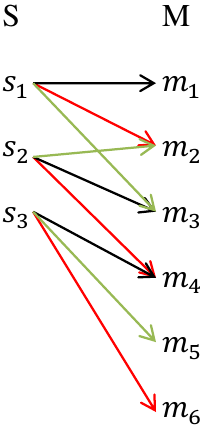
\includegraphics[scale=0.5]{a_codes}
\end{figure}
\begin{equation*}
  E = \left\{ {e}_{1},{e}_{2} \right\} \cup \left\{{e}_{3}\right\}
\end{equation*}
\begin{equation*}
{e}_{1}:\qquad
{s}_{1}\rightarrow {m}_{1},\qquad
{s}_{2}\rightarrow {m}_{3},\qquad
{s}_{3}\rightarrow {m}_{4} \qquad
\end{equation*}

\begin{equation*}
{e}_{2}:\qquad
{s}_{1}\rightarrow {m}_{3},\qquad
{s}_{2}\rightarrow {m}_{2},\qquad
{s}_{3}\rightarrow {m}_{5} \qquad
\end{equation*}

\begin{equation*}
{e}_{3}:\qquad
{s}_{1}\rightarrow {m}_{2},\qquad
{s}_{2}\rightarrow {m}_{4},\qquad
{s}_{3}\rightarrow {m}_{6} \qquad
\end{equation*}

Проверяем условия:
\begin{enumerate}
  \item
    \begin{equation*}
      M=\bigcup\limits_{e}e\left(S\right)
    \end{equation*}
    Не выполняется: ${m}_{6}$ не достижимо.

    \begin{equation*}
      {e}_{1}\left(S\right)=\left\{{m}_{1},{m}_{3},{m}_{4}\right\},\qquad
      {e}_{2}\left(S\right)=\left\{{m}_{2},{m}_{3},{m}_{5}\right\}
    \end{equation*}
    Но с ${e}_{3}$ будет выполняться: 
    \begin{equation*}
      {e}_{3}\left(S\right)=\left\{{m}_{2},{m}_{4},{m}_{6}\right\}
    \end{equation*}

  \item
    ${\forall}s:{f}_{e}\left(e\left(S\right)\right)=S$ --- выполняется

  \item
    $\left| M \right| > \left| S \right|$ --- таки да

  \item
    ${\forall}m:1<\left|E\left(m\right)\right|<\left|E\right|$

    $E\left({m}_{1}\right)=\left\{{e}_{1}\right\}$ --- очень плохо

    $E\left({m}_{2}\right)=\left\{{e}_{2},{e}_{3}\right\}$

    $E\left({m}_{3}\right)=\left\{{e}_{1},{e}_{2}\right\}$

    $E\left({m}_{4}\right)=\left\{{e}_{1},{e}_{3}\right\}$

    $E\left({m}_{5}\right)=\left\{{e}_{2}\right\}$ --- очень плохо

    $E\left({m}_{6}\right)=\left\{{e}_{3}\right\}$ --- очень плохо

    Если аналитик пронаблюдает  ${m}_{1}$, ${m}_{5}$, ${m}_{6}$ он будет точно
    знать, что используется отображение  ${e}_{1}$,  ${e}_{2}$, или 
    ${e}_{3}$ соответственно (и узнаёт состояние, которое защищалось). 

    $\Rightarrow$ Легко сделать обман/подделку (потому что
    известно кодирующее отображение).

    Если же {\textbar}E(m){\textbar}={\textbar}E{\textbar} и m раньше
    не посылалось, то аналитик просто отправляет m Бобу, и тот его с
    радостью принимает, потому что какое бы ни использовалось кодирующее
    отображение, m будет правильным сообщением.

  \item
    $\forall m: \bigcap\limits_{e \in E\left( m \right)} e\left( S \right) = \left\{ m \right\}$
    не выполняется уже для $m_1$:

    \begin{equation*}
      \bigcap\limits_{e \in E\left( m \right)} e\left( S \right)
        = \left\{{m}_{1},{m}_{3},{m}_{4}\right\}
    \end{equation*}

    Аналитик ловит сообщение $m$ и обнаруживает, что

    \begin{equation*}
      \bigcap\limits_{e \in E\left( m \right)} e\left( S \right)
      = \left\{m,m'\right\} \Rightarrow m'
    \end{equation*}
    тоже будет правильным сообщением, хотя $e$ осталось неизвестным.
\end{enumerate}

! Для того, чтобы аналитик не смог подделать сообщение путём случайного
выбора, необходимо, чтобы 
${\forall}c:\left\{m:{f}_{e}\left(m\right)=0\right\}$ было большим.

В этом случае случайный выбор $m$ попадет на $0$ с большой вероятностью.

$A$-код без секретности --- не скрывает состояние $S$. 

В этом случае можно и представить его в виде $A$-кода с аутентификатором: 
 $M{\subseteq}S\times A$.

$m=(s, a)$, $a$ --- аутентификатор.

Пусть  $\overline{e}: S \rightarrow A$ --- функция вычисления аутентификатора.

\subsection{Построение $A$-кода с аутентификатором по $A$-коду без секретности}

Обозначим:

\begin{equation*}
  \begin{split}
    M\left(S\right)
      &=\left\{ m\in M\mid\exists e \in E:e\left(S\right)=m\right\} \\
    \mu_{s}
      &=\left|M\left(S\right)\right| \\
    \mu
      &=\max\limits_{s}{\mu}_{s}
  \end{split}
\end{equation*}
Зная $\mu$, выбираем произвольное множество 
$A = \left\{{a}_{1},{\dots},{a}_{\mu }\right\}$, которое будем
использовать в качестве аутентификаторов.

Новое множество сообщений  $M=\left\{{m}_{1},{\dots},{m}_{\gamma
}\right\}{\subseteq}S\times A$  ?

Тогда  $M\left(S\right)=\left\{{m}_{{i}_{1}},{\dots},{m}_{{i}_{{\mu
}_{s}}}\right\}$,  ${\mu }_{{i}_{j}}={e}_{j}(S)$  ?

Положим  $\overline{e_j\left( S \right)}={a}_{j}$,
$j=\overline{{1,{\dots},{\mu }_{s}}}$ и поставим взаимно-однозначное
соответствие: $M\left(S\right)\leftrightarrow {M}_{s}$

\begin{equation*}
  {M}_{s}
  =\left\{\left({s}_{1},{a}_{1}\right),
          \left({s}_{1}, {a}_{2}\right), {\dots},(s_1,{a}_{\mu_s})\right\}
\end{equation*}
Тогда новое множество сообщений $\overline{M}=\bigcup_s M_s$

\begin{example}
  \begin{equation*}
    S=\left\{H,T\right\},\qquad
    M=\left\{{m}_{1},{\dots},{m}_{5}\right\},\qquad
    E=\left\{{e}_{1},{\dots},{e}_{6}\right\}
  \end{equation*}

  \begin{center}
    \begin{tabular}{|*{6}{c|}}
      \hline
      \backslashbox{e}{m} & $m_1$ & $m_2$ & $m_3$ & $m_4$ & $m_5$ \\
      \hline
      $e_1$               &  $H$  &  $T$  &  $0$  &  $0$  & $0$   \\
      \hline              
      $e_2$               &  $0$  &  $0$  &  $H$  &  $T$  & $0$   \\
      \hline              
      $e_3$               &  $0$  &  $0$  &  $H$  &  $0$  & $T$   \\
      \hline              
      $e_4$               &  $H$  &  $0$  &  $0$  &  $T$  & $0$   \\
      \hline
      $e_5$               &  $0$  &  $T$  &  $H$  &  $0$  & $0$   \\
      \hline
      $e_6$               &  $H$  &  $0$  &  $0$  &  $0$  & $T$   \\
      \hline
    \end{tabular}
  \end{center}

  Секретности нет: каждое  ${m}_{i}$ получается либо только из Н, либо
  только из Т.

  \begin{equation*}
    \begin{split}
      M\left(H\right)&=\left\{{m}_{1},{m}_{3}\right\} \\
      M\left(T\right)&=\{{m}_{2},{m}_{4},{m}_{5}\} \\
      \mu&=3 \\
      {\mu }_{H}&=2 \\
      {\mu }_{T}&=3
    \end{split}
  \end{equation*}
   $A=\left\{{a}_{1},{a}_{2},{a}_{3}\right\}$ --- аутентификаторы
   $\left\{a,b,c\right\}$
  Тогда
  \begin{equation*}
    \begin{split}
      {M}_{H}&=\left\{\left(H,a\right),\left(H,b\right)\right\} \\
      {M}_{T}&=\{\left(T,a\right),\left(T,b\right),(T,c)\} \\
      \overline{M}&={M}_{H} \cup {M}_{T} \subseteq S\times A
    \end{split}
  \end{equation*}
  Отображение $M\rightarrow \overline{M}$:
  \begin{equation*}
    \begin{split}
    {m}_{1}\rightarrow \left(H,a\right),\qquad
    {m}_{2}\rightarrow \left(T,a\right),\qquad
    {m}_{3}\rightarrow \left(H,b\right),\\
    {m}_{4}\rightarrow \left(T,b\right),\qquad
    {m}_{5}\rightarrow \left(T,c\right).
    \end{split}
  \end{equation*}
\end{example}
